\documentclass[tikz]{standalone}
\usepackage[utf8]{inputenc}
\usepackage{amsmath, amssymb, latexsym}
\usepackage{color}

\usepackage{tikz}
\usetikzlibrary{decorations.pathreplacing}
\usetikzlibrary{fadings}
\usetikzlibrary{positioning}

\begin{document}
	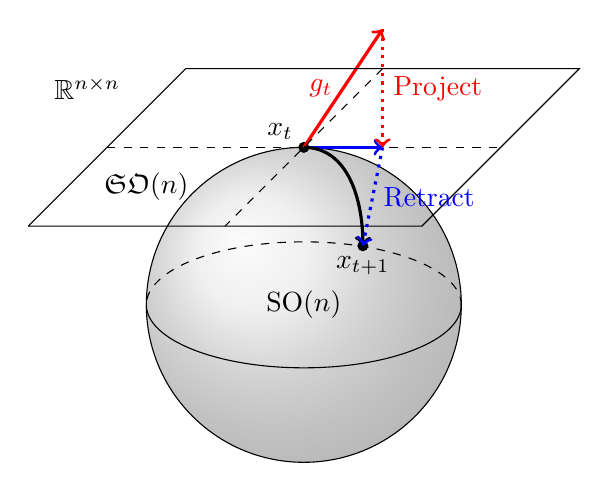
\begin{tikzpicture}


\shade[ball color = gray!40, opacity = 0.4] (0,0) circle (2);
\draw (0,0) circle (2);
\draw (-2,0) arc (180:360:2 and 0.8);
\draw[dashed] (2 ,0) arc (0:180:2 and 0.8);
\node at (0,0){SO$(n)$};

\fill[fill=black] (0,2) circle (2pt);
\node at (-0.3,2.2) {$x_t$};
\draw[draw=red,solid,->,line width=0.4mm] (0,2 ) -- node[left]{\color{red}$g_t$} (1,3.5);
\node at (-2,1.5){$\mathfrak{SO}(n)$};
\node at (-2.75,2.75){$\mathbb{R}^{n\times n}$};
\def\xshift{0}
\def\yshift{-0.5}
\draw[] (-3.5+\xshift,1.5+\yshift) -- (-1.5+\xshift,3.5+\yshift) -- (3.5+\xshift,3.5+\yshift) -- (1.5+\xshift,1.5+\yshift) -- (-3.5+\xshift,1.5+\yshift);
\draw[dashed] (-2.5+\xshift,2.5+\yshift) -- (2.5+\xshift,2.5+\yshift);
\draw[dashed] (1+\xshift,3.5+\yshift) -- (-1+\xshift,1.5+\yshift);

\fill[fill=black] (0.75,0.75) circle (2pt);
\node at (0.75,0.5) {$x_{t+1}$};

\draw[draw=blue,solid,->,line width=0.4mm] (0,2 ) -- %node[above]{\color{blue}P}
(1,2);
\draw[draw=black,solid,->,line width=0.4mm] (0,2 ) to[out=0,in=90] %node[above]{\color{blue}P}
(0.75,0.75);
\draw[draw=blue,dotted,->,line width=0.4mm] (1,2 ) -- node[right]{\color{blue}Retract}
(0.75,0.75);
\draw[draw=red,dotted,->,line width=0.4mm] (1,3.5 ) -- node[right]{\color{red}Project} (1,2);
\end{tikzpicture}
%
\end{document}
